\documentclass[a4paper,12pt]{article}

%% Language and font encodings
\usepackage[english]{babel}
\usepackage[utf8x]{inputenc}
\usepackage[T1]{fontenc}
\usepackage{tikz}

%% Sets page size and margins
\usepackage[a4paper,top=3cm,bottom=2cm,left=3cm,right=3cm,marginparwidth=1.00cm]{geometry}

%% Useful packages
\usepackage{amsmath}
\usepackage{graphicx}
\usepackage[colorinlistoftodos]{todonotes}
\usepackage[colorlinks=true, allcolors=blue]{hyperref}

\title{Gravitation: Revision lecture - Exercises}
%\author{}
\date{}
\begin{document}
\maketitle

(H1 students only need to do the questions marked with a * at the end.)\\
\begin{enumerate}
\item The orbital radius of the Moon around the Earth is $3.84 × 10^8$ m. The mass of the Moon is $7.34 × 10^{22}$ kg. The mass of the Earth is $6.0 × 10^{24}$ kg. 

\begin{enumerate}
\item Calculate the force of gravity exerted by the Earth on the Moon. *
\item Determine the orbital period of the Moon around the Earth in days. Assume that the orbit is circular with the Earth at the centre. *
\item It is a fact that an observer on the Earth sees the same face of the Moon all the time. Deduce the rotational period of the Moon about its own axis. *
\item Determine the gravitational field strength at a point that lies along the line between Earth and Moon, such that the distance of this point from the centre of the Moon is one-tenth of the distance between the centres of the Earth and the Moon.
\item Determine the gravitational potential at the point specified in (d).
\end{enumerate}

%..........Q2...................
\vspace{1cm}

\item An unmanned spacecraft is orbiting the planet Mars at a distance of 300 km above its surface. The radius of Mars is 3390 km. The mass of the spacecraft is 2180 kg. 

\begin{enumerate}
\item It is known that the acceleration due to gravity on the surface of Mars is 3.71 m s$^{-2}$. Determine the mass of Mars. 
\item Calculate the tangential speed and period of the spacecraft while it is in orbit at an altitude of 300 km above the Martian surface. (For H1: The mass of Mars is 6.42 × $10^{23}$ kg.) *
 \item Calculate the gravitational field strength at any point along the circular orbit in (b). 
\item Calculate the gravitational force acting on a 20.0 g mass inside the spacecraft. State the centripetal acceleration of this mass. *
\item For a particular mission, it is required for the orbiting spacecraft to be directly above a robotic rover on the Martian equator at all times. Determine the radius of this \emph{synchronous orbit}. Mars rotates once about its axis every 1.026 Earth days.* \\ 

The spacecraft uses its rocket engines to adjust its orbit from its initial orbit in (b) to the final synchronous orbit in (e).\\ 

\item Determine the gravitational potential at any point in the initial orbit that is 300 km above the surface. 
\item Determine the work that must be done by the spacecraft’s rocket engines to change its orbital radius from that in (b) to that in (e).
\item If the spacecraft in synchronous orbit comes to rest relative to Mars, determine the speed with which it will hit the surface. 
\item Due to a malfunction, the rocket fuel inside the spacecraft in synchronous orbit ignites and explodes, destroying the spacecraft and causing pieces of metal to fly off in all directions. Determine the minimum speed that a piece of metal must have immediately after the explosion for it to escape the Martian gravity permanently.
\end{enumerate}



\vspace{1cm}

\item Halley's comet orbits the Sun along an elliptical path.\\

\begin{figure}[h]
    \centering
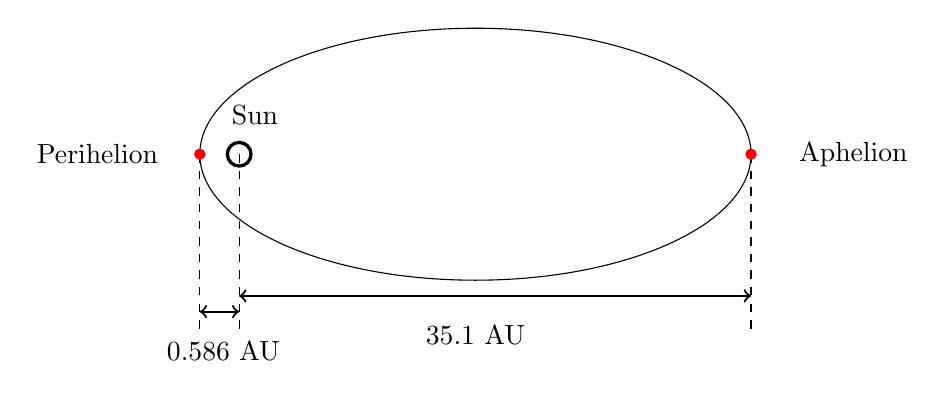
\begin{tikzpicture}
%\draw[help lines, color=gray!30, thick] (-4.9,-4.9) grid (4.9,4.9);
\draw {(0,0) ellipse (3.5 and 1.6)};
\draw [very thick] (-3,0) circle (0.15cm);
\draw [<->, thick] (-3.5,-2) -- (-3,-2);
\draw [dashed] (-3.5,0) -- (-3.5,-2.3);
\draw [dashed] (-3.0,0) -- (-3.0,-2.3);
\node (r_min) at (-3.2,-2.5) {0.586 AU};
\draw [<->, thick] (-3,-1.8) -- (3.5,-1.8) ;
\draw [dashed] (3.5,0) -- (3.5,-2.3);
\node (r_max) at (0,-2.3) {35.1 AU};
\node (sun) at (-2.8,0.5) {Sun};
\filldraw [very thick,color=red] (-3.5,0) circle (0.05cm);
\node (perihelion) at (-4.8,0) {Perihelion};
\filldraw [very thick,color=red] (3.5,0) circle (0.05cm);
\node (aphelion) at (4.8,0) {Aphelion};
%\draw[->,ultra thick] (-5,0)--(5,0) node[right]{$x$};
%\draw[->,ultra thick] (0,-5)--(0,5) node[above]{$y$};
\end{tikzpicture}
    \caption{Trajectory of Halley's comet around the Sun}
    \label{fig:halley}
\end{figure}

The closest distance that Halley’s comet gets to the Sun in its periodic elliptical orbit is 0.586 AU. The greatest distance that it gets away from the Sun 35.1 AU.\\ (1 AU = Distance between Sun and Earth = $1.50 × 10^{11}$ m). 


\begin{enumerate}
\item Calculate the gravitational potential $\phi_1$  at the point at which Halley’s comet is closest to the Sun (perihelion).
\item Calculate the gravitational potential $\phi_2$ at the point at which Halley’s comet is farthest from the Sun (aphelion).
\item It is known that the speed of the comet at its perihelion is 70.56 km s$^{-1}$. Determine its speed at the aphelion. Ignore the gravitational effect of all other celestial bodies. 
\end{enumerate}
\end{enumerate}


\end{document}